\documentclass{article} % For LaTeX2e
\usepackage{iclr2026_conference,times}

%%%%% NEW MATH DEFINITIONS %%%%%

\usepackage{amsmath,amsfonts,bm}

% Mark sections of captions for referring to divisions of figures
\newcommand{\figleft}{{\em (Left)}}
\newcommand{\figcenter}{{\em (Center)}}
\newcommand{\figright}{{\em (Right)}}
\newcommand{\figtop}{{\em (Top)}}
\newcommand{\figbottom}{{\em (Bottom)}}
\newcommand{\captiona}{{\em (a)}}
\newcommand{\captionb}{{\em (b)}}
\newcommand{\captionc}{{\em (c)}}
\newcommand{\captiond}{{\em (d)}}

% Highlight a newly defined term
\newcommand{\newterm}[1]{{\bf #1}}


% Figure reference, lower-case.
\def\figref#1{figure~\ref{#1}}
% Figure reference, capital. For start of sentence
\def\Figref#1{Figure~\ref{#1}}
\def\twofigref#1#2{figures \ref{#1} and \ref{#2}}
\def\quadfigref#1#2#3#4{figures \ref{#1}, \ref{#2}, \ref{#3} and \ref{#4}}
% Section reference, lower-case.
\def\secref#1{section~\ref{#1}}
% Section reference, capital.
\def\Secref#1{Section~\ref{#1}}
% Reference to two sections.
\def\twosecrefs#1#2{sections \ref{#1} and \ref{#2}}
% Reference to three sections.
\def\secrefs#1#2#3{sections \ref{#1}, \ref{#2} and \ref{#3}}
% Reference to an equation, lower-case.
\def\eqref#1{equation~\ref{#1}}
% Reference to an equation, upper case
\def\Eqref#1{Equation~\ref{#1}}
% A raw reference to an equation---avoid using if possible
\def\plaineqref#1{\ref{#1}}
% Reference to a chapter, lower-case.
\def\chapref#1{chapter~\ref{#1}}
% Reference to an equation, upper case.
\def\Chapref#1{Chapter~\ref{#1}}
% Reference to a range of chapters
\def\rangechapref#1#2{chapters\ref{#1}--\ref{#2}}
% Reference to an algorithm, lower-case.
\def\algref#1{algorithm~\ref{#1}}
% Reference to an algorithm, upper case.
\def\Algref#1{Algorithm~\ref{#1}}
\def\twoalgref#1#2{algorithms \ref{#1} and \ref{#2}}
\def\Twoalgref#1#2{Algorithms \ref{#1} and \ref{#2}}
% Reference to a part, lower case
\def\partref#1{part~\ref{#1}}
% Reference to a part, upper case
\def\Partref#1{Part~\ref{#1}}
\def\twopartref#1#2{parts \ref{#1} and \ref{#2}}

\def\ceil#1{\lceil #1 \rceil}
\def\floor#1{\lfloor #1 \rfloor}
\def\1{\bm{1}}
\newcommand{\train}{\mathcal{D}}
\newcommand{\valid}{\mathcal{D_{\mathrm{valid}}}}
\newcommand{\test}{\mathcal{D_{\mathrm{test}}}}

\def\eps{{\epsilon}}


% Random variables
\def\reta{{\textnormal{$\eta$}}}
\def\ra{{\textnormal{a}}}
\def\rb{{\textnormal{b}}}
\def\rc{{\textnormal{c}}}
\def\rd{{\textnormal{d}}}
\def\re{{\textnormal{e}}}
\def\rf{{\textnormal{f}}}
\def\rg{{\textnormal{g}}}
\def\rh{{\textnormal{h}}}
\def\ri{{\textnormal{i}}}
\def\rj{{\textnormal{j}}}
\def\rk{{\textnormal{k}}}
\def\rl{{\textnormal{l}}}
% rm is already a command, just don't name any random variables m
\def\rn{{\textnormal{n}}}
\def\ro{{\textnormal{o}}}
\def\rp{{\textnormal{p}}}
\def\rq{{\textnormal{q}}}
\def\rr{{\textnormal{r}}}
\def\rs{{\textnormal{s}}}
\def\rt{{\textnormal{t}}}
\def\ru{{\textnormal{u}}}
\def\rv{{\textnormal{v}}}
\def\rw{{\textnormal{w}}}
\def\rx{{\textnormal{x}}}
\def\ry{{\textnormal{y}}}
\def\rz{{\textnormal{z}}}

% Random vectors
\def\rvepsilon{{\mathbf{\epsilon}}}
\def\rvtheta{{\mathbf{\theta}}}
\def\rva{{\mathbf{a}}}
\def\rvb{{\mathbf{b}}}
\def\rvc{{\mathbf{c}}}
\def\rvd{{\mathbf{d}}}
\def\rve{{\mathbf{e}}}
\def\rvf{{\mathbf{f}}}
\def\rvg{{\mathbf{g}}}
\def\rvh{{\mathbf{h}}}
\def\rvu{{\mathbf{i}}}
\def\rvj{{\mathbf{j}}}
\def\rvk{{\mathbf{k}}}
\def\rvl{{\mathbf{l}}}
\def\rvm{{\mathbf{m}}}
\def\rvn{{\mathbf{n}}}
\def\rvo{{\mathbf{o}}}
\def\rvp{{\mathbf{p}}}
\def\rvq{{\mathbf{q}}}
\def\rvr{{\mathbf{r}}}
\def\rvs{{\mathbf{s}}}
\def\rvt{{\mathbf{t}}}
\def\rvu{{\mathbf{u}}}
\def\rvv{{\mathbf{v}}}
\def\rvw{{\mathbf{w}}}
\def\rvx{{\mathbf{x}}}
\def\rvy{{\mathbf{y}}}
\def\rvz{{\mathbf{z}}}

% Elements of random vectors
\def\erva{{\textnormal{a}}}
\def\ervb{{\textnormal{b}}}
\def\ervc{{\textnormal{c}}}
\def\ervd{{\textnormal{d}}}
\def\erve{{\textnormal{e}}}
\def\ervf{{\textnormal{f}}}
\def\ervg{{\textnormal{g}}}
\def\ervh{{\textnormal{h}}}
\def\ervi{{\textnormal{i}}}
\def\ervj{{\textnormal{j}}}
\def\ervk{{\textnormal{k}}}
\def\ervl{{\textnormal{l}}}
\def\ervm{{\textnormal{m}}}
\def\ervn{{\textnormal{n}}}
\def\ervo{{\textnormal{o}}}
\def\ervp{{\textnormal{p}}}
\def\ervq{{\textnormal{q}}}
\def\ervr{{\textnormal{r}}}
\def\ervs{{\textnormal{s}}}
\def\ervt{{\textnormal{t}}}
\def\ervu{{\textnormal{u}}}
\def\ervv{{\textnormal{v}}}
\def\ervw{{\textnormal{w}}}
\def\ervx{{\textnormal{x}}}
\def\ervy{{\textnormal{y}}}
\def\ervz{{\textnormal{z}}}

% Random matrices
\def\rmA{{\mathbf{A}}}
\def\rmB{{\mathbf{B}}}
\def\rmC{{\mathbf{C}}}
\def\rmD{{\mathbf{D}}}
\def\rmE{{\mathbf{E}}}
\def\rmF{{\mathbf{F}}}
\def\rmG{{\mathbf{G}}}
\def\rmH{{\mathbf{H}}}
\def\rmI{{\mathbf{I}}}
\def\rmJ{{\mathbf{J}}}
\def\rmK{{\mathbf{K}}}
\def\rmL{{\mathbf{L}}}
\def\rmM{{\mathbf{M}}}
\def\rmN{{\mathbf{N}}}
\def\rmO{{\mathbf{O}}}
\def\rmP{{\mathbf{P}}}
\def\rmQ{{\mathbf{Q}}}
\def\rmR{{\mathbf{R}}}
\def\rmS{{\mathbf{S}}}
\def\rmT{{\mathbf{T}}}
\def\rmU{{\mathbf{U}}}
\def\rmV{{\mathbf{V}}}
\def\rmW{{\mathbf{W}}}
\def\rmX{{\mathbf{X}}}
\def\rmY{{\mathbf{Y}}}
\def\rmZ{{\mathbf{Z}}}

% Elements of random matrices
\def\ermA{{\textnormal{A}}}
\def\ermB{{\textnormal{B}}}
\def\ermC{{\textnormal{C}}}
\def\ermD{{\textnormal{D}}}
\def\ermE{{\textnormal{E}}}
\def\ermF{{\textnormal{F}}}
\def\ermG{{\textnormal{G}}}
\def\ermH{{\textnormal{H}}}
\def\ermI{{\textnormal{I}}}
\def\ermJ{{\textnormal{J}}}
\def\ermK{{\textnormal{K}}}
\def\ermL{{\textnormal{L}}}
\def\ermM{{\textnormal{M}}}
\def\ermN{{\textnormal{N}}}
\def\ermO{{\textnormal{O}}}
\def\ermP{{\textnormal{P}}}
\def\ermQ{{\textnormal{Q}}}
\def\ermR{{\textnormal{R}}}
\def\ermS{{\textnormal{S}}}
\def\ermT{{\textnormal{T}}}
\def\ermU{{\textnormal{U}}}
\def\ermV{{\textnormal{V}}}
\def\ermW{{\textnormal{W}}}
\def\ermX{{\textnormal{X}}}
\def\ermY{{\textnormal{Y}}}
\def\ermZ{{\textnormal{Z}}}

% Vectors
\def\vzero{{\bm{0}}}
\def\vone{{\bm{1}}}
\def\vmu{{\bm{\mu}}}
\def\vtheta{{\bm{\theta}}}
\def\va{{\bm{a}}}
\def\vb{{\bm{b}}}
\def\vc{{\bm{c}}}
\def\vd{{\bm{d}}}
\def\ve{{\bm{e}}}
\def\vf{{\bm{f}}}
\def\vg{{\bm{g}}}
\def\vh{{\bm{h}}}
\def\vi{{\bm{i}}}
\def\vj{{\bm{j}}}
\def\vk{{\bm{k}}}
\def\vl{{\bm{l}}}
\def\vm{{\bm{m}}}
\def\vn{{\bm{n}}}
\def\vo{{\bm{o}}}
\def\vp{{\bm{p}}}
\def\vq{{\bm{q}}}
\def\vr{{\bm{r}}}
\def\vs{{\bm{s}}}
\def\vt{{\bm{t}}}
\def\vu{{\bm{u}}}
\def\vv{{\bm{v}}}
\def\vw{{\bm{w}}}
\def\vx{{\bm{x}}}
\def\vy{{\bm{y}}}
\def\vz{{\bm{z}}}

% Elements of vectors
\def\evalpha{{\alpha}}
\def\evbeta{{\beta}}
\def\evepsilon{{\epsilon}}
\def\evlambda{{\lambda}}
\def\evomega{{\omega}}
\def\evmu{{\mu}}
\def\evpsi{{\psi}}
\def\evsigma{{\sigma}}
\def\evtheta{{\theta}}
\def\eva{{a}}
\def\evb{{b}}
\def\evc{{c}}
\def\evd{{d}}
\def\eve{{e}}
\def\evf{{f}}
\def\evg{{g}}
\def\evh{{h}}
\def\evi{{i}}
\def\evj{{j}}
\def\evk{{k}}
\def\evl{{l}}
\def\evm{{m}}
\def\evn{{n}}
\def\evo{{o}}
\def\evp{{p}}
\def\evq{{q}}
\def\evr{{r}}
\def\evs{{s}}
\def\evt{{t}}
\def\evu{{u}}
\def\evv{{v}}
\def\evw{{w}}
\def\evx{{x}}
\def\evy{{y}}
\def\evz{{z}}

% Matrix
\def\mA{{\bm{A}}}
\def\mB{{\bm{B}}}
\def\mC{{\bm{C}}}
\def\mD{{\bm{D}}}
\def\mE{{\bm{E}}}
\def\mF{{\bm{F}}}
\def\mG{{\bm{G}}}
\def\mH{{\bm{H}}}
\def\mI{{\bm{I}}}
\def\mJ{{\bm{J}}}
\def\mK{{\bm{K}}}
\def\mL{{\bm{L}}}
\def\mM{{\bm{M}}}
\def\mN{{\bm{N}}}
\def\mO{{\bm{O}}}
\def\mP{{\bm{P}}}
\def\mQ{{\bm{Q}}}
\def\mR{{\bm{R}}}
\def\mS{{\bm{S}}}
\def\mT{{\bm{T}}}
\def\mU{{\bm{U}}}
\def\mV{{\bm{V}}}
\def\mW{{\bm{W}}}
\def\mX{{\bm{X}}}
\def\mY{{\bm{Y}}}
\def\mZ{{\bm{Z}}}
\def\mBeta{{\bm{\beta}}}
\def\mPhi{{\bm{\Phi}}}
\def\mLambda{{\bm{\Lambda}}}
\def\mSigma{{\bm{\Sigma}}}

% Tensor
\DeclareMathAlphabet{\mathsfit}{\encodingdefault}{\sfdefault}{m}{sl}
\SetMathAlphabet{\mathsfit}{bold}{\encodingdefault}{\sfdefault}{bx}{n}
\newcommand{\tens}[1]{\bm{\mathsfit{#1}}}
\def\tA{{\tens{A}}}
\def\tB{{\tens{B}}}
\def\tC{{\tens{C}}}
\def\tD{{\tens{D}}}
\def\tE{{\tens{E}}}
\def\tF{{\tens{F}}}
\def\tG{{\tens{G}}}
\def\tH{{\tens{H}}}
\def\tI{{\tens{I}}}
\def\tJ{{\tens{J}}}
\def\tK{{\tens{K}}}
\def\tL{{\tens{L}}}
\def\tM{{\tens{M}}}
\def\tN{{\tens{N}}}
\def\tO{{\tens{O}}}
\def\tP{{\tens{P}}}
\def\tQ{{\tens{Q}}}
\def\tR{{\tens{R}}}
\def\tS{{\tens{S}}}
\def\tT{{\tens{T}}}
\def\tU{{\tens{U}}}
\def\tV{{\tens{V}}}
\def\tW{{\tens{W}}}
\def\tX{{\tens{X}}}
\def\tY{{\tens{Y}}}
\def\tZ{{\tens{Z}}}


% Graph
\def\gA{{\mathcal{A}}}
\def\gB{{\mathcal{B}}}
\def\gC{{\mathcal{C}}}
\def\gD{{\mathcal{D}}}
\def\gE{{\mathcal{E}}}
\def\gF{{\mathcal{F}}}
\def\gG{{\mathcal{G}}}
\def\gH{{\mathcal{H}}}
\def\gI{{\mathcal{I}}}
\def\gJ{{\mathcal{J}}}
\def\gK{{\mathcal{K}}}
\def\gL{{\mathcal{L}}}
\def\gM{{\mathcal{M}}}
\def\gN{{\mathcal{N}}}
\def\gO{{\mathcal{O}}}
\def\gP{{\mathcal{P}}}
\def\gQ{{\mathcal{Q}}}
\def\gR{{\mathcal{R}}}
\def\gS{{\mathcal{S}}}
\def\gT{{\mathcal{T}}}
\def\gU{{\mathcal{U}}}
\def\gV{{\mathcal{V}}}
\def\gW{{\mathcal{W}}}
\def\gX{{\mathcal{X}}}
\def\gY{{\mathcal{Y}}}
\def\gZ{{\mathcal{Z}}}

% Sets
\def\sA{{\mathbb{A}}}
\def\sB{{\mathbb{B}}}
\def\sC{{\mathbb{C}}}
\def\sD{{\mathbb{D}}}
% Don't use a set called E, because this would be the same as our symbol
% for expectation.
\def\sF{{\mathbb{F}}}
\def\sG{{\mathbb{G}}}
\def\sH{{\mathbb{H}}}
\def\sI{{\mathbb{I}}}
\def\sJ{{\mathbb{J}}}
\def\sK{{\mathbb{K}}}
\def\sL{{\mathbb{L}}}
\def\sM{{\mathbb{M}}}
\def\sN{{\mathbb{N}}}
\def\sO{{\mathbb{O}}}
\def\sP{{\mathbb{P}}}
\def\sQ{{\mathbb{Q}}}
\def\sR{{\mathbb{R}}}
\def\sS{{\mathbb{S}}}
\def\sT{{\mathbb{T}}}
\def\sU{{\mathbb{U}}}
\def\sV{{\mathbb{V}}}
\def\sW{{\mathbb{W}}}
\def\sX{{\mathbb{X}}}
\def\sY{{\mathbb{Y}}}
\def\sZ{{\mathbb{Z}}}

% Entries of a matrix
\def\emLambda{{\Lambda}}
\def\emA{{A}}
\def\emB{{B}}
\def\emC{{C}}
\def\emD{{D}}
\def\emE{{E}}
\def\emF{{F}}
\def\emG{{G}}
\def\emH{{H}}
\def\emI{{I}}
\def\emJ{{J}}
\def\emK{{K}}
\def\emL{{L}}
\def\emM{{M}}
\def\emN{{N}}
\def\emO{{O}}
\def\emP{{P}}
\def\emQ{{Q}}
\def\emR{{R}}
\def\emS{{S}}
\def\emT{{T}}
\def\emU{{U}}
\def\emV{{V}}
\def\emW{{W}}
\def\emX{{X}}
\def\emY{{Y}}
\def\emZ{{Z}}
\def\emSigma{{\Sigma}}

% entries of a tensor
% Same font as tensor, without \bm wrapper
\newcommand{\etens}[1]{\mathsfit{#1}}
\def\etLambda{{\etens{\Lambda}}}
\def\etA{{\etens{A}}}
\def\etB{{\etens{B}}}
\def\etC{{\etens{C}}}
\def\etD{{\etens{D}}}
\def\etE{{\etens{E}}}
\def\etF{{\etens{F}}}
\def\etG{{\etens{G}}}
\def\etH{{\etens{H}}}
\def\etI{{\etens{I}}}
\def\etJ{{\etens{J}}}
\def\etK{{\etens{K}}}
\def\etL{{\etens{L}}}
\def\etM{{\etens{M}}}
\def\etN{{\etens{N}}}
\def\etO{{\etens{O}}}
\def\etP{{\etens{P}}}
\def\etQ{{\etens{Q}}}
\def\etR{{\etens{R}}}
\def\etS{{\etens{S}}}
\def\etT{{\etens{T}}}
\def\etU{{\etens{U}}}
\def\etV{{\etens{V}}}
\def\etW{{\etens{W}}}
\def\etX{{\etens{X}}}
\def\etY{{\etens{Y}}}
\def\etZ{{\etens{Z}}}

% The true underlying data generating distribution
\newcommand{\pdata}{p_{\rm{data}}}
% The empirical distribution defined by the training set
\newcommand{\ptrain}{\hat{p}_{\rm{data}}}
\newcommand{\Ptrain}{\hat{P}_{\rm{data}}}
% The model distribution
\newcommand{\pmodel}{p_{\rm{model}}}
\newcommand{\Pmodel}{P_{\rm{model}}}
\newcommand{\ptildemodel}{\tilde{p}_{\rm{model}}}
% Stochastic autoencoder distributions
\newcommand{\pencode}{p_{\rm{encoder}}}
\newcommand{\pdecode}{p_{\rm{decoder}}}
\newcommand{\precons}{p_{\rm{reconstruct}}}

\newcommand{\laplace}{\mathrm{Laplace}} % Laplace distribution

\newcommand{\E}{\mathbb{E}}
\newcommand{\Ls}{\mathcal{L}}
\newcommand{\R}{\mathbb{R}}
\newcommand{\emp}{\tilde{p}}
\newcommand{\lr}{\alpha}
\newcommand{\reg}{\lambda}
\newcommand{\rect}{\mathrm{rectifier}}
\newcommand{\softmax}{\mathrm{softmax}}
\newcommand{\sigmoid}{\sigma}
\newcommand{\softplus}{\zeta}
\newcommand{\KL}{D_{\mathrm{KL}}}
\newcommand{\Var}{\mathrm{Var}}
\newcommand{\standarderror}{\mathrm{SE}}
\newcommand{\Cov}{\mathrm{Cov}}
% Wolfram Mathworld says $L^2$ is for function spaces and $\ell^2$ is for vectors
% But then they seem to use $L^2$ for vectors throughout the site, and so does
% wikipedia.
\newcommand{\normlzero}{L^0}
\newcommand{\normlone}{L^1}
\newcommand{\normltwo}{L^2}
\newcommand{\normlp}{L^p}
\newcommand{\normmax}{L^\infty}

\newcommand{\parents}{Pa} % See usage in notation.tex. Chosen to match Daphne's book.

\DeclareMathOperator*{\argmax}{arg\,max}
\DeclareMathOperator*{\argmin}{arg\,min}

\DeclareMathOperator{\sign}{sign}
\DeclareMathOperator{\Tr}{Tr}
\let\ab\allowbreak


\usepackage{hyperref}
\usepackage{url}
\usepackage{graphicx}
\usepackage{booktabs}
\usepackage{amsmath}

\title{Reading the Market: News-Augmented Regime Discovery \\ via Unsupervised Representation Learning}

\author{Yixiang Huang \\
University of Chicago \,/\, Toyota Technological Institute at Chicago \\
\texttt{yixianghuang@uchicago.edu}}

\newcommand{\fix}{\marginpar{FIX}}
\newcommand{\new}{\marginpar{NEW}}

\iclrfinalcopy
\begin{document}

\maketitle

\begin{abstract}
Hidden-Markov regime models for financial markets operate on price-derived
features alone, so the regimes they recover are reactive: they change only
after information has been absorbed by prices. We ask whether unsupervised
representations of financial news yield regimes that are better separated and
more persistent than a price-only baseline. On 6{,}262 trading days of the
S\&P~500 (2000--2024) we compare 18 clustering pipelines spanning price-only,
news-only, and price-plus-news feature stacks, built from four text
representations (sentiment scalars, latent Dirichlet allocation, BERTopic, and
FinBERT) and two news corpora (firm-level press releases and aggregate macro
news). A held-out grid search over 180 configurations then tunes the
representation, dimensionality reduction, clustering method, and number of
regimes. News augmentation raises the silhouette score by 34\% over the
price-only hidden Markov model (0.202 to 0.270) while keeping regimes inside an
interpretable multi-month persistence band. Aggregate macro news outperforms
firm-level press releases, and the tuned configuration (BERTopic + PCA-95\% +
$k$-means, $K=5$) reaches a silhouette of 0.279 at a 202-day mean regime
duration. Adding price features back on top stabilizes regimes further
(224 days) at negligible cost to separation.
\end{abstract}

\section{Introduction}

A \emph{market regime} is a persistent state of the financial market
characterized by distinct return and risk behavior, such as a calm bull market
or a high-volatility crisis. The standard tool for recovering regimes is the
hidden Markov model (HMM) of \citet{hamilton1989}, which treats the regime as a
latent discrete state driving observed price features such as returns and
volatility \citep{ang2012}. Because these models read only from prices, the
regimes they discover are reactive by construction: a regime boundary can move
only once new information has already changed returns or volatility.

Financial news is a natural candidate for a complementary, possibly earlier,
signal. Prior work shows that news sentiment and news topics carry information
about returns and aggregate risk \citep{tetlock2007, glasserman2019,
bybee2024}. That work is mostly supervised or forecasting-oriented. We instead
ask an \emph{unsupervised} question: without any labeled regimes, do
representations of news produce a regime \emph{structure} that is better
separated and more stable than the structure recovered from prices alone?

We study this question as a controlled comparison of clustering pipelines. The
contributions are:
\begin{itemize}
  \item A systematic comparison of four text representations (sentiment
  scalars, LDA, BERTopic, FinBERT) crossed with three clustering algorithms
  (Gaussian mixtures, HMMs, $k$-means) for unsupervised regime discovery, against a
  price-only HMM baseline.
  \item A comparison of two news corpora at different granularity: firm-level
  press releases and aggregate macro news.
  \item A four-axis evaluation protocol that scores each pipeline on
  statistical fit, clustering geometry, temporal stability, and financial
  interpretability, rather than on any single number.
  \item A reproducibility finding: full-covariance HMMs collapse to an
  absorbing state on high-dimensional fused features, which a switch to
  diagonal covariance fixes.
\end{itemize}

\section{Related work}

\textbf{Regime models.} \citet{hamilton1989} introduced the Markov-switching
model for nonstationary economic series; the approach is now standard for
markets \citep{ang2012}. These models use price- and macro-derived observables.
We keep the same latent-state view but ask whether text representations improve
the recovered states under unsupervised evaluation.

\textbf{News and markets.} \citet{tetlock2007} links media sentiment to
returns; \citet{glasserman2019} build an ``unusual news'' indicator that
forecasts market stress; and \citet{bybee2024} show that news topics track the
business cycle. These studies predict a known target (returns, volatility, or
recession dates). Our setting has no target: we cluster, then ask whether the
clusters are geometrically and economically coherent.

\textbf{Text representations.} We use latent Dirichlet allocation
\citep{blei2003}, BERTopic \citep{grootendorst2022}, and FinBERT
\citep{araci2019} embeddings \citep{reimers2019} as off-the-shelf encoders, and
study how each behaves as input to clustering rather than proposing a new
encoder.

\section{Data}
\label{sec:data}

\textbf{Market features.} We build five daily features for the S\&P~500 over
2000--2024 from CRSP and FRED: the daily return, 21-day realized volatility,
the VIX, the term spread (10Y minus 2Y Treasury yield), and the credit spread
(Baa minus Aaa corporate yield). After aligning all sources we retain 6{,}262
trading days.

\textbf{News corpora.} We pair the market series with two RavenPack news
corpora at complementary granularity. The \emph{firm-level} corpus (Dow Jones
press releases, ``DJPR'') is filtered to US entities (\texttt{entity\_type =
COMP}) with relevance $\geq 75$. The \emph{macro} corpus (Dow Jones Global
Macro) carries about 24 million rows across 27 yearly partitions and captures
aggregate attention to rates, commodities, currencies, and global events; it
begins in 2000. For each corpus we aggregate to daily series of sentiment
statistics (mean and standard deviation of composite sentiment, article count,
positive/negative fractions, and net sentiment).

\section{Methods}
\label{sec:methods}

Each pipeline maps raw inputs to a daily sequence of regime labels through five
stages: assemble features, smooth, represent text, reduce dimensionality, and
cluster.

\textbf{Text representations.} We compute four representations of each news
corpus. \emph{Scalar} is the five-dimensional vector of daily sentiment
statistics. \emph{LDA} \citep{blei2003} gives a $K\in\{15,20\}$-dimensional
topic distribution per day. \emph{BERTopic} \citep{grootendorst2022} yields
about 20 topic weights from contextual embeddings. \emph{FinBERT}
\citep{araci2019} provides a 768-dimensional embedding, averaged to a daily
vector.

\textbf{Smoothing.} Daily news is noisy, so we apply a per-representation
rolling mean before clustering: 35 days for scalar features, 30 for LDA, 21 for
BERTopic, and 10 for FinBERT. Topic representations are already daily
aggregates and need less smoothing than the raw scalars.

\textbf{Feature stacks.} We enumerate three pathways: \emph{price-only} (the
five market features), \emph{news-only} (one or both corpora, in one of the
text representations), and \emph{hybrid} (price plus news). Crossing pathways,
representations, and corpora gives the 18 main pipelines.

\textbf{Dimensionality reduction.} Before clustering we optionally reduce the
assembled feature stack with PCA (retaining 95\% of variance) or UMAP
\citep{mcinnes2018} to 10 dimensions.

\textbf{Clustering.} We cluster with three algorithms: a Gaussian mixture model
(GMM), an HMM, and $k$-means. For the GMM and HMM the number of regimes $K$ is
selected by the Bayesian information criterion and log-likelihood,
respectively; for $k$-means we test $K\in\{3,4,5\}$. The HMM uses a sticky
initialization (transition diagonal 0.85), 300 EM iterations, and the best of
five random seeds by log-likelihood.

\textbf{A covariance failure mode.} On fused stacks with dimension $\geq 10$, a
full-covariance HMM collapses to an absorbing state: one regime absorbs almost
all days and the mean regime duration runs away to 894 days, far outside any
interpretable range. Switching to a diagonal covariance whenever the feature
dimension is at least 10 recovers multi-month regimes, and we adopt it as the
default.

\section{Evaluation protocol}
\label{sec:eval}

A clustering has no ground-truth labels, so we score each pipeline on four
complementary axes rather than one number.

\textbf{Statistical fit.} For the probabilistic models we report the
log-likelihood and the Bayesian and Akaike information criteria,
$\mathrm{BIC} = -2\log L + k\log N$, which penalize parameter count.

\textbf{Clustering geometry.} We report the silhouette coefficient
\citep{rousseeuw1987} (higher is better separation) and the Davies--Bouldin
index \citep{davies1979} (DBI; lower is better). Unless noted, both are computed
on a common standardized feature space so that pipelines are comparable.

\textbf{Temporal stability.} We report the mean regime duration in days and a
rolling adjusted Rand index (ARI) over a 1250-day window, which measures how
stable the regime assignment is to perturbing the data window. We treat a mean
duration of 60--365 days as the interpretable band: shorter regimes flicker too
fast to name, and longer ones are too coarse to be useful.

\textbf{Financial interpretability.} For each regime we compute the annualized
Sharpe ratio, maximum drawdown, and average VIX, and report the best regime's
Sharpe as a summary of whether the discovered states separate good and bad
market conditions.

\section{Experiments and results}
\label{sec:results}

\subsection{Baseline}
The price-only HMM recovers five regimes with a 95-day mean duration and a
clean crisis state: one regime carries an average VIX of 41 and a $-51\%$
maximum drawdown, while the calmest regime has a Sharpe of 2.0 and an average
VIX of 13. The baseline therefore separates market conditions well by financial
measures, but its short 95-day regimes change quickly because they react to
price moves.

\subsection{Does news help?}
Table~\ref{tab:master} compares the baseline with the news-augmented pipelines.
News augmentation raises the silhouette from 0.202 (price-only HMM) to 0.270
(macro sentiment HMM), a 34\% improvement, and lowers the Davies--Bouldin index.
The improvement is not specific to one representation: the scalar, LDA, and
BERTopic representations on the macro corpus all beat the price baseline on
silhouette. Figure~\ref{fig:scatter} shows the silhouette/Sharpe trade-off
across all main pipelines: text-only pipelines (green) tend to cluster at high
silhouette, while hybrid pipelines (orange) keep the baseline's higher Sharpe.

\begin{table}[t]
\caption{Master evaluation. Arrows give the preferred direction.
$\star$ marks configurations selected by the grid search of
Section~\ref{sec:tuning}. Silhouette and DBI for the two tuned pipelines are
measured in the reduced (PCA-95\%) space in which they were selected; the other
rows use the common standardized space of Section~\ref{sec:eval}.}
\label{tab:master}
\begin{center}
\begin{tabular}{lccccc}
\toprule
\textbf{Pipeline} & \textbf{Sil.}\,$\uparrow$ & \textbf{DBI}\,$\downarrow$ & \textbf{Dur. (d)} & \textbf{ARI}\,$\uparrow$ & \textbf{Sharpe} \\
\midrule
Price-only HMM (baseline)        & 0.202 & 1.48 & \phantom{0}95 & 0.447 & 2.02 \\
DJPR sentiment HMM               & 0.284 & 1.26 & \phantom{0}44 & 0.383 & 0.80 \\
Macro sentiment HMM $\star$      & 0.270 & 1.27 & 174 & 0.239 & 0.65 \\
DJPR topic-vector HMM            & 0.261 & 1.49 & \phantom{0}70 & 0.278 & 0.64 \\
Dual-corpus sentiment fusion     & 0.245 & 1.42 & \phantom{0}49 & 0.268 & 1.00 \\
Tuned news fusion $\star$        & 0.279 & 0.95 & 202 & 0.31\phantom{0} & 0.78 \\
Tuned full stack (+ price) $\star$ & 0.272 & 0.92 & 224 & 0.33\phantom{0} & 1.21 \\
\bottomrule
\end{tabular}
\end{center}
\end{table}

\subsection{Aggregate news beats firm-level news}
A higher silhouette is not enough on its own. The DJPR sentiment HMM has the
highest silhouette in the table (0.284) but a 44-day mean duration, so its
regimes flicker too fast to interpret as market states. The macro sentiment
HMM, by contrast, lands inside the interpretable band at 174 days while still
beating the baseline on silhouette. Aggregate attention to rates, commodities,
and global events is a steadier regime signal than the firm-level press-release
stream, whose day-to-day sentiment is dominated by idiosyncratic company news.

\subsection{Tuning the pipeline}
\label{sec:tuning}
We then run a grid search over 180 configurations (two feature stacks $\times$
90 settings) along four axes: text representation (LDA-15, LDA-20, BERTopic, and
FinBERT under PCA-20, PCA-50, or UMAP-10), post-stack dimensionality reduction
(none, PCA-95\%, UMAP-10), clustering algorithm (GMM, HMM, $k$-means), and $K$.
We select the configuration with the highest silhouette \emph{subject to} a
mean duration in the 60--365-day band. This constraint matters: the highest raw
silhouettes (0.55--0.66) all come from FinBERT + UMAP configurations whose
regimes last 270--1250 days, well past the interpretable range, and whose
silhouette is measured in the very UMAP space that UMAP optimizes for
separation, so it is not comparable to the PCA or raw-space scores. The best
configuration within the band is BERTopic + PCA-95\% + $k$-means with $K=5$,
which reaches a silhouette of 0.279 at a 202-day mean duration.

\subsection{Price stabilizes news-driven regimes}
Adding the five market features on top of the tuned news fusion (the
``full stack'' row) increases the mean regime duration from 202 to 224 days at
negligible cost to silhouette (0.279 to 0.272) and raises the best-regime
Sharpe from 0.78 to 1.21. Price acts as a low-frequency anchor that steadies the
news-driven regimes against narrative noise.

\subsection{Regime characterization}
Figure~\ref{fig:timelines} overlays the regime sequences on the cumulative
S\&P~500. The news-augmented pipelines recover the same crisis structure as the
price baseline---the dot-com bust, the global financial crisis, and the COVID
crash all sit at regime boundaries---but with smoother, longer segments. The
tuned news fusion, for example, places its 2000--2004 regime at an average VIX
of 25 and a negative Sharpe, and its post-2021 regime in the rate-hike era,
matching the economic narrative without ever seeing prices.

\begin{figure}[t]
\begin{center}
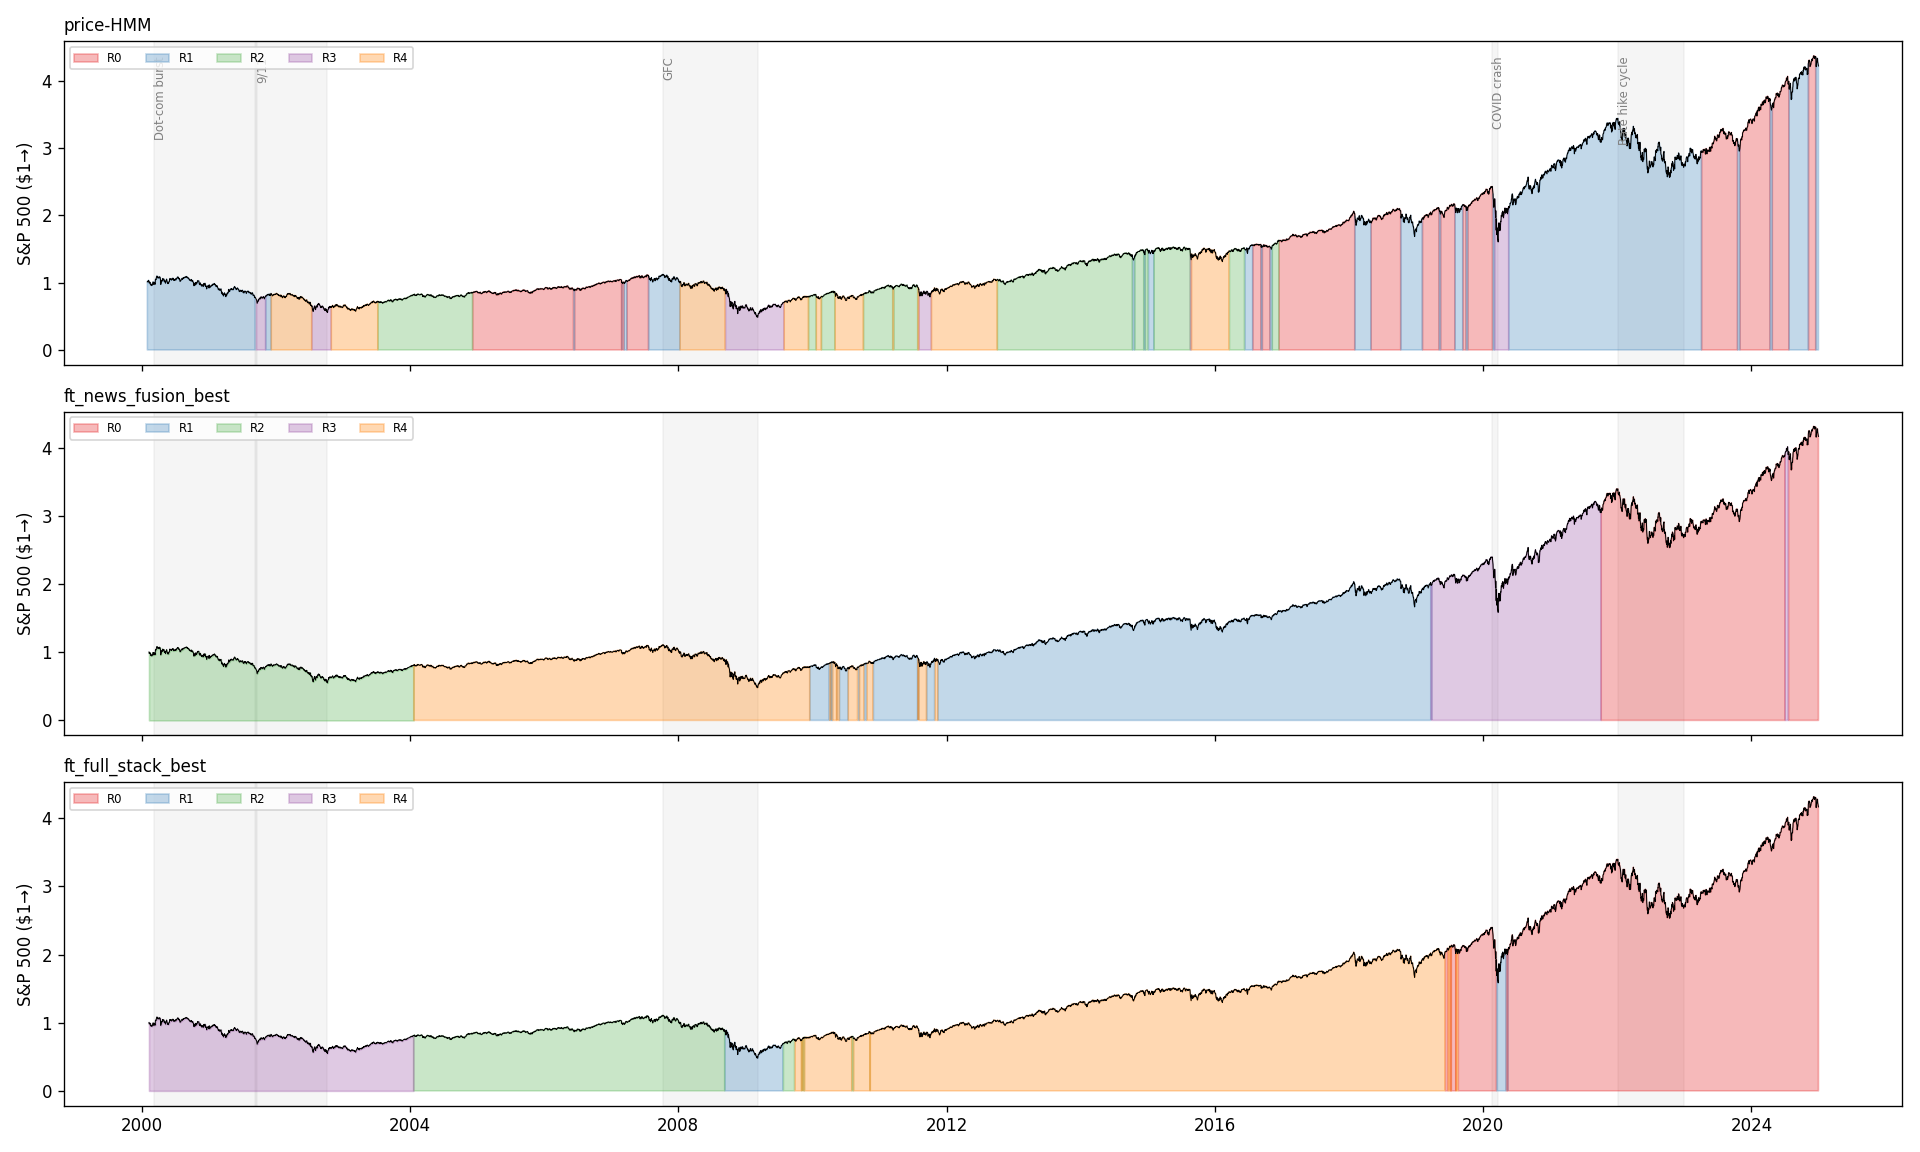
\includegraphics[width=0.9\linewidth]{figs/regime_tour_4panel.png}
\end{center}
\caption{Regime timelines on the cumulative S\&P~500 (\$1 growth). Top:
price-only HMM baseline (95-day mean duration). Middle: tuned news fusion
(BERTopic + PCA-95\% + $k$-means, $K=5$; 202-day duration). Bottom: tuned full
stack (+ market features; 224-day duration). Shaded vertical bands mark known
crises. News-augmented regimes capture the same crisis dynamics with shifted,
smoother boundaries.}
\label{fig:timelines}
\end{figure}

\begin{figure}[t]
\begin{center}
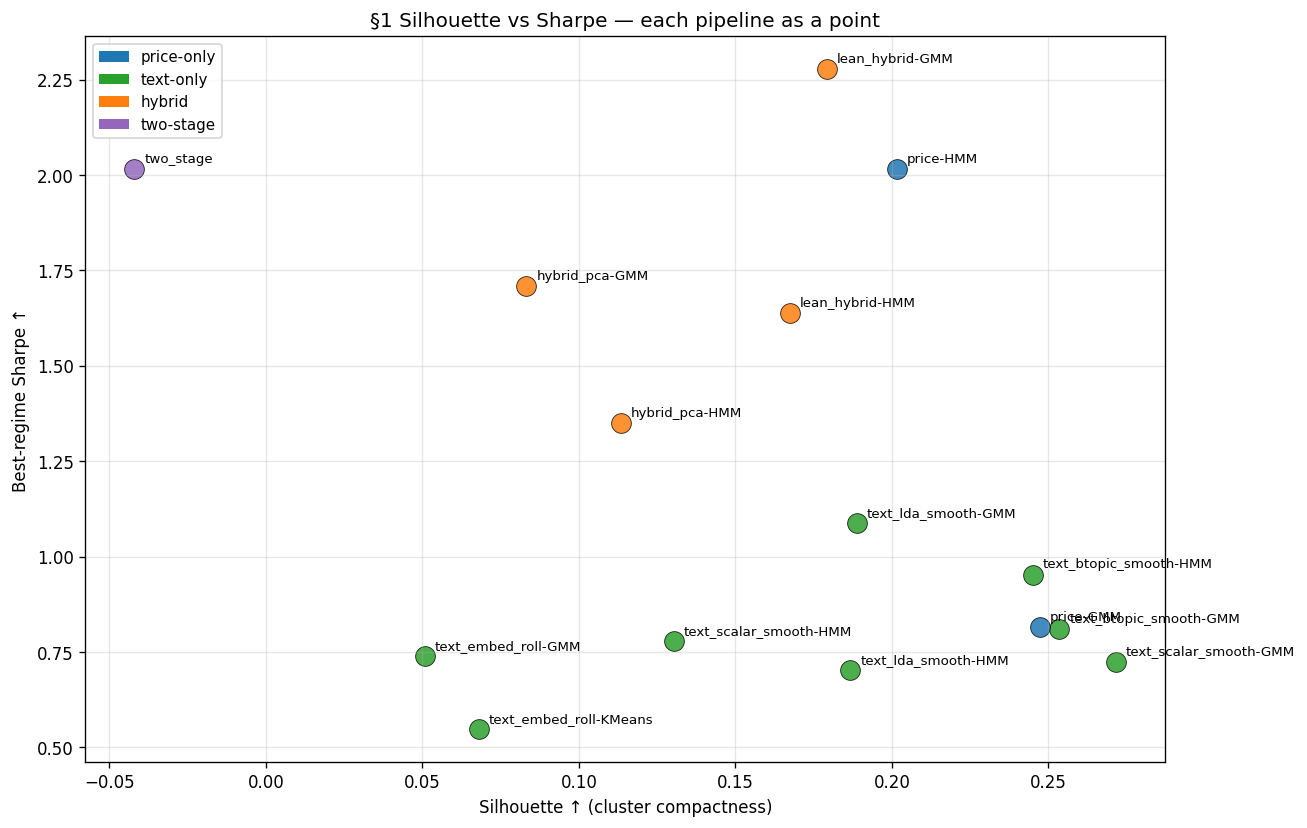
\includegraphics[width=0.62\linewidth]{figs/final_sil_sharpe_scatter.png}
\end{center}
\caption{Silhouette versus best-regime Sharpe for the main pipelines, colored
by feature family. Text-only pipelines reach the highest silhouettes; hybrid
pipelines retain the price baseline's higher Sharpe. Silhouette is computed on
the common standardized space.}
\label{fig:scatter}
\end{figure}

\section{Discussion}

The results support a specific, limited claim: unsupervised news
representations recover regimes that are better separated (higher silhouette,
lower DBI) and, on the macro corpus, more persistent than the price-only
baseline, while still aligning with known crises and with sensible per-regime
risk. They do \emph{not} show that news leads prices; establishing that would
require an explicit lead--lag test, which we leave to future work. The tuning
experiment also makes a measurement caveat concrete: silhouette computed in a
reduced space, especially a UMAP space, is not comparable across spaces, and a
high silhouette paired with a multi-year regime is degenerate rather than good.
Reporting clustering geometry alongside a persistence band keeps the comparison
honest.

\section{Limitations and future work}

The evaluation is in-sample: every pipeline is fit on the full 2000--2024
window. A walk-forward out-of-sample check using a persisted HMM and
\texttt{predict()} on a held-out post-2020 window would test stability under
true generalization. We also report point estimates of silhouette without a
bootstrap confidence interval, so pairwise differences between close pipelines
are not formally significant. The macro corpus begins in 2000, so we cannot
probe earlier regimes. Promising extensions are a replication of the
\citet{glasserman2019} unusual-news indicator as an external benchmark, and
changepoint-aware adaptive smoothing in place of fixed windows.

\subsubsection*{Author contributions}
This is a solo project. Y.~Huang designed the study, implemented the full
pipeline and evaluation, ran all experiments, and wrote the report.

\subsubsection*{Reproducibility statement}
The pipeline runs end to end with \texttt{python run\_pipeline.py} (stages
01--08 with incremental caching); the grid search lives under
\texttt{finetuning/}. Section~\ref{sec:methods} states the smoothing windows,
HMM initialization, and covariance rule needed to reproduce the regimes.

\bibliography{references}
\bibliographystyle{iclr2026_conference}

\appendix
\section{Appendix}

\subsection{Full pipeline and grid specification}
The 18 main pipelines enumerate the price-only, news-only, and hybrid pathways
across the four text representations and two corpora. The grid search runs 90
configurations per feature stack (news-only fusion and full stack): six text
representations (LDA-15, LDA-20, BERTopic, and FinBERT under PCA-20, PCA-50, or
UMAP-10), three post-stack reductions (none, PCA-95\%, UMAP-10), and five
clustering setups (GMM and HMM with auto-$K$, and $k$-means at $K\in\{3,4,5\}$),
for 180 configurations in total. Per-configuration results, including the
degenerate high-silhouette UMAP configurations discussed in
Section~\ref{sec:tuning}, are stored in
\texttt{\_data/ft\_\{news\_fusion,full\_stack\}\_results.parquet}.

\end{document}
